
\begin{frame}
\frametitle{Klassifikation}

\begin{center}
\begin{tabular}{llll}
Klasse&Bedingung&Beispiel&Anwendung\\
\hline
elliptisch &$\begin{aligned}P&=n\mathstrut\end{aligned}$
	&$\displaystyle \Delta u=f                                $
		&Potential\\
&	&	&Eigenwertproblem\\
\hline
parabolisch&%$P=n-1, Z=1$
$\begin{aligned}P&=n-1\mathstrut\\Z&=1\mathstrut\end{aligned}$
	&$\displaystyle \frac{\partial u}{\partial t}=\Delta u    $
		&W"armeleitung\\
\hline
hyperbolisch&%$P=n-1, N=1$
$\begin{aligned}P&=n-1\mathstrut\\N&=1\mathstrut\end{aligned}$
	&$\displaystyle \frac{\partial^2 u}{\partial t^2}=\Delta u$
		&Wellen\\
\hline
\end{tabular}
\end{center}

Klasse verr"at:
\begin{itemize}
\item Charakter der L"osung: Schwingungen, exponentielles Abklingen
\item Welches L"osungsverfahren geeignet ist
\end{itemize}

\end{frame}

\begin{frame}
\frametitle{Elliptische PDGL}
\begin{center}
\includegraphics{../../skript/images/kausal-1.pdf}
\end{center}
\end{frame}

\begin{frame}
\frametitle{Quasilineare PDGL 1. Ordnung}
\begin{center}
\includegraphics{../../skript/images/kausal-2.pdf}
\end{center}
\end{frame}

\begin{frame}
\frametitle{Wellen}
\begin{center}
\includegraphics[width=\hsize]{wellen-1.pdf}
\end{center}
\end{frame}

\begin{frame}
\frametitle{Wellen}
\begin{center}
\includegraphics[width=\hsize]{wellen-2.pdf}
\end{center}
\end{frame}

\begin{frame}
\frametitle{Wellen}
\begin{center}
\includegraphics[width=\hsize]{wellen-3.pdf}
\end{center}
\end{frame}

\begin{frame}
\frametitle{Wellen}
\begin{center}
\includegraphics[width=\hsize]{wellen-4.pdf}
\end{center}
\end{frame}

\begin{frame}
\frametitle{Wellen}
\begin{center}
\includegraphics[width=\hsize]{wellen-5.pdf}
\end{center}
\end{frame}

\begin{frame}
\frametitle{Wellen}
\begin{center}
\includegraphics[width=\hsize]{wellen-6.pdf}
\end{center}
\end{frame}

\begin{frame}
\frametitle{Wellen}
\begin{center}
\includegraphics[width=\hsize]{wellen-7.pdf}
\end{center}
\end{frame}

\begin{frame}
\frametitle{Wellen}
\begin{center}
\includegraphics[width=\hsize]{wellen-8.pdf}
\end{center}
\end{frame}

\begin{frame}
\frametitle{Wellen}
\begin{center}
\includegraphics[width=\hsize]{wellen-9.pdf}
\end{center}
\end{frame}

\begin{frame}
\frametitle{Wellen}
\begin{center}
\includegraphics[width=\hsize]{wellen-10.pdf}
\end{center}
\end{frame}

\begin{frame}
\frametitle{Wellen}
\begin{center}
\includegraphics[width=\hsize]{wellen-11.pdf}
\end{center}
\end{frame}

\begin{frame}
\frametitle{Wellen}
\begin{center}
\includegraphics[width=\hsize]{wellen-12.pdf}
\end{center}
\end{frame}

\begin{frame}
\frametitle{Wellen}
\begin{center}
\includegraphics[width=\hsize]{wellen-13.pdf}
\end{center}
\end{frame}

\begin{frame}
\frametitle{Wellen}
\begin{center}
\includegraphics[width=\hsize]{wellen-14.pdf}
\end{center}
\end{frame}

\begin{frame}
\frametitle{Wellen}
\begin{center}
\includegraphics[width=\hsize]{wellen-15.pdf}
\end{center}
\end{frame}

\begin{frame}
\frametitle{Wellen}
\begin{center}
\includegraphics[width=\hsize]{wellen-16.pdf}
\end{center}
\end{frame}

\begin{frame}
\frametitle{Wellen}
\begin{center}
\includegraphics[width=\hsize]{wellen-17.pdf}
\end{center}
\end{frame}

\begin{frame}
\frametitle{Wellen}
\begin{center}
\includegraphics[width=\hsize]{wellen-18.pdf}
\end{center}
\end{frame}

\begin{frame}
\frametitle{Wellen}
\begin{center}
\includegraphics[width=\hsize]{wellen-19.pdf}
\end{center}
\end{frame}

\begin{frame}
\frametitle{Wellen}
\begin{center}
\includegraphics[width=\hsize]{wellen-20.pdf}
\end{center}
\end{frame}

\begin{frame}
\frametitle{Wellen}
\begin{center}
\includegraphics[width=\hsize]{wellen-21.pdf}
\end{center}
\end{frame}

\begin{frame}
\frametitle{Wellen}
\begin{center}
\includegraphics[width=\hsize]{wellen-22.pdf}
\end{center}
\end{frame}

\begin{frame}
\frametitle{Wellen}
\begin{center}
\includegraphics[width=\hsize]{wellen-23.pdf}
\end{center}
\end{frame}

\begin{frame}
\begin{center}
\includegraphics[height=0.9\vsize]{wdom-1.pdf}
\end{center}
\end{frame}

\begin{frame}
\begin{center}
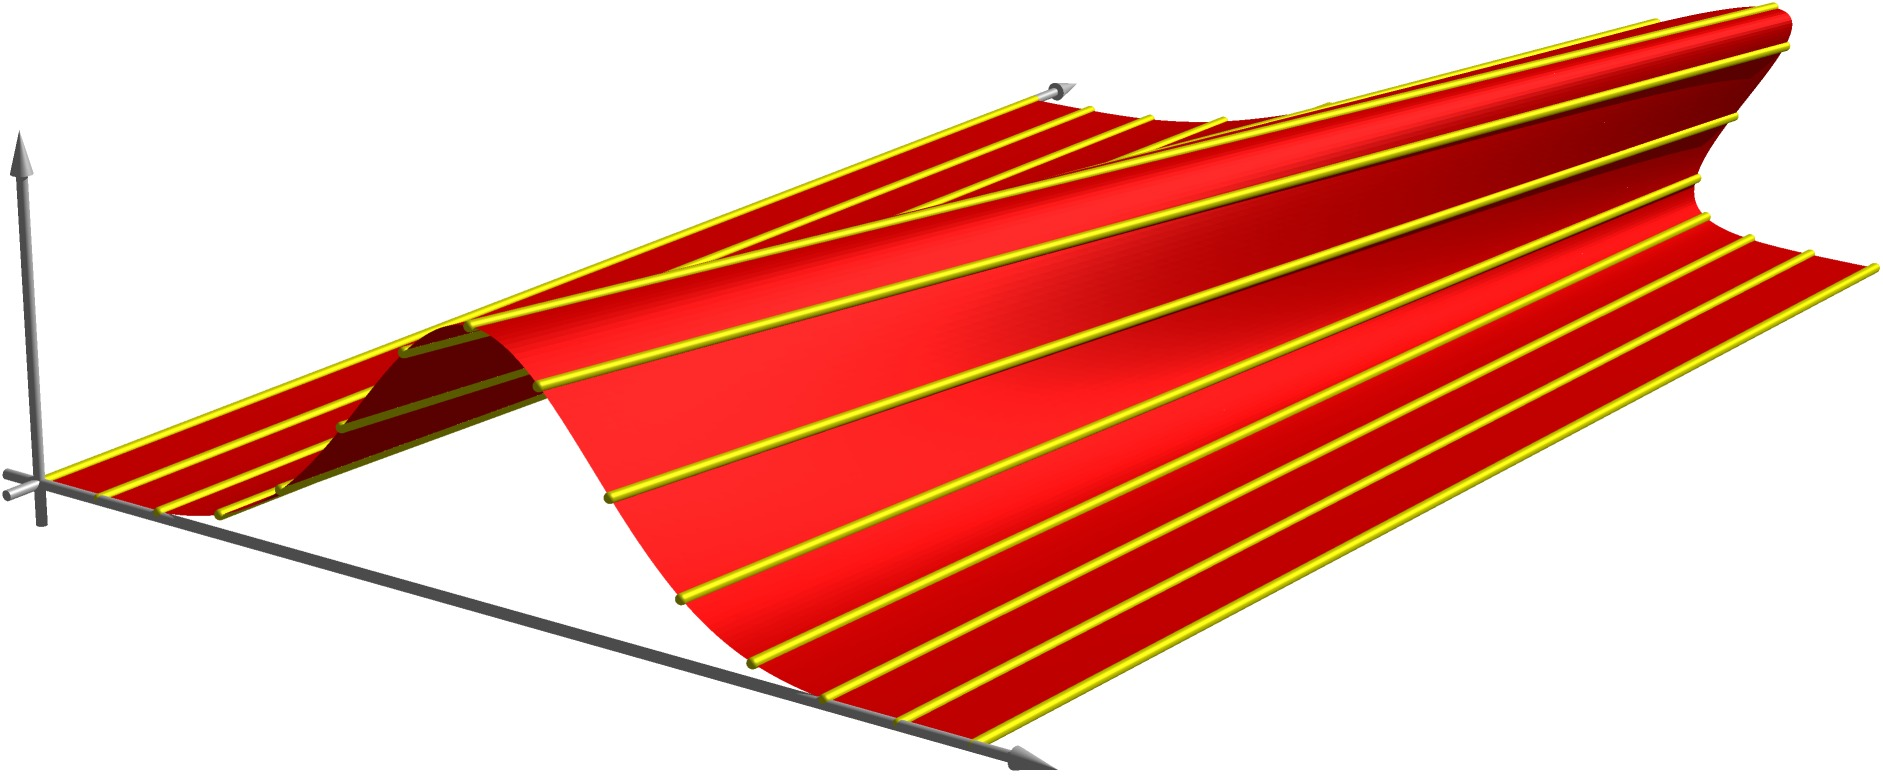
\includegraphics[width=\hsize]{welle.jpg}
\end{center}
\end{frame}

\begin{frame}
\begin{center}
\includegraphics[width=\hsize]{wellegrid.jpg}
\end{center}
\end{frame}

\begin{frame}
\frametitle{Wellengleichung}
Kr"ummung in beiden Richtungen gleich:
\[
\text{Kr"ummung in $x$-Richtung}
=
\text{Kr"ummung in $t$-Richtung}
\]
Kr"ummung ist zweite Ableitung:
\[
\frac{\partial^2 u}{\partial x^2}
=
\frac{\partial^2 u}{\partial t^2}
\]
$\Rightarrow$
Wellengleichung
\bigskip

{\bf Prinzip:}
Welle = L"osung der Wellengleichung
\end{frame}

\begin{frame}
\frametitle{d'Alembert-Operator}
Wellengleichung mit Geschwindigkeit $c$:
\[
\frac{\partial^2u}{\partial x^2}
+
\frac{\partial^2u}{\partial y^2}
+
\frac{\partial^2u}{\partial z^2}
-
\frac1{c^2}
\frac{\partial^2u}{\partial t^2}
=
0
\]
Operatorschreibweise mit d'Alembert-Operator:
\[
\square 
=
\frac{\partial^2}{\partial x^2}
+
\frac{\partial^2}{\partial y^2}
+
\frac{\partial^2}{\partial z^2}
-
\frac1{c^2}
\frac{\partial^2}{\partial t^2}
\qquad
\Rightarrow
\qquad
\square u=0
\]
\end{frame}

\begin{frame}
\frametitle{d'Alembert-L"osung}
1-dim Wellengleichung, Ausbreitungsgeschwindigkeit $a$:
\begin{enumerate}
\item
Nach rechts laufende Welle:
\[
u_{\text{rechts}}(x-at)
\]
\item
Nach links laufende Welle:
\[
u_{\text{links}}(x+at)
\]
\end{enumerate}
\pause
\[
\Rightarrow
\]
Allgemeine L"osung
\[
u(x,t)
=
u_{\text{rechts}}(x-at)
+
u_{\text{links}}(x+at)
\]
\end{frame}


\begin{frame}
\frametitle{Hyperbolische PDGL}

\begin{itemize}[<+->]
\item
Prototyp: Wellengleichung
\item
endliche Ausbreitungsgeschwindigkeit
\item
Jeder Randwert hat ein durch die Ausbreitungsgeschwindigkeit
definiertes Einflussgebiet
\end{itemize}
\pause
\bigskip

{\bf Aufgabe:}
Finde die Einflussgebiete f"ur eine beliebige hyperbolische PDGL
\bigskip

\pause
{\bf L"osung mit d'Alembert:}
Punkt $(x,t)$ wird von $(x-at,0)$ und $(x+at,0)$ beeinflusst.

\end{frame}

\begin{frame}
\frametitle{Quasilineare PDGL 1. Ordnung}
\begin{center}
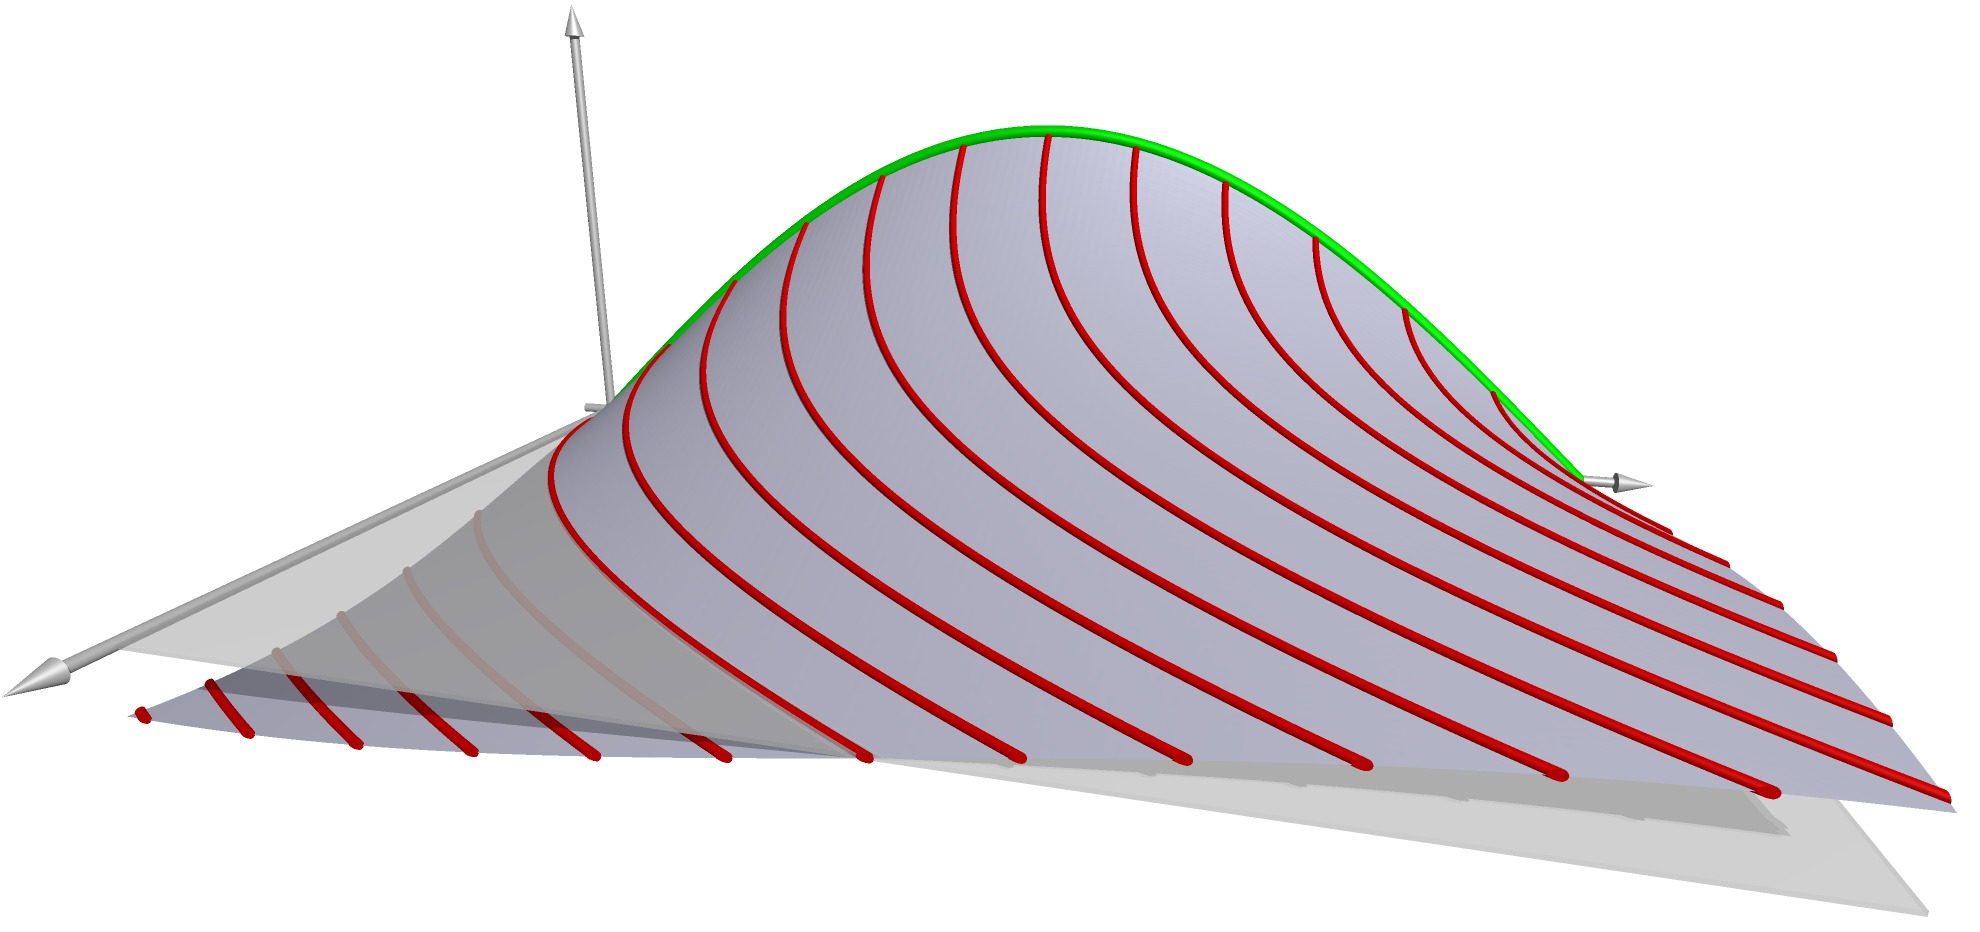
\includegraphics[width=\hsize]{../../skript/3d/sol.jpg}
\end{center}
\end{frame}

\begin{frame}
\frametitle{Quasilineare PDGL 1. Ordnung}

{\bf Prinzip:} Steigung der Anfangskurve und PDGL legen Steigung in Richtung
``quer'' zur Anfangskurve fest.
\pause
\bigskip

Charakteristiken:
\[
t\mapsto \left\{\begin{aligned}
x(t)\\
y(t)\\
u(t)
\end{aligned}\right.
\]
{\bf L"osung:} Anfangskurve entlang von Charakteristiken transportieren.
\pause

\begin{definition}
Charakteristiken sind Kurven, die {\color{red}nicht} als Anfangskurven f"ur ein
Cauchy-Problem geeignet sind.
\end{definition}

\begin{theorem}
Die L"osungsfl"achen wird von Charakteristiken erzeugt.
\end{theorem}

\end{frame}

\begin{frame}
\frametitle{Hyperbolische PDGL}
Partielle Differentialgleichung zweiter Ordnung
\[
Lu
=
a\frac{\partial^2 u}{\partial x^2}
+
2b \frac{\partial^2 u}{\partial x\,\partial y}
+
c\frac{\partial^2 u}{\partial y^2}
+
d\frac{\partial u}{\partial x}
+
e\frac{\partial u}{\partial y}
+
fu=g
\]
mit
\[
\left|\begin{matrix}
a&b\\b&c
\end{matrix}\right|
=ac-b^2 < 0
\quad\Leftrightarrow\quad
\text{$L$ hyperbolisch}
\]
im Gebiet $\Omega$.
\end{frame}

\begin{frame}
\frametitle{Streifen}

Anfangsdaten f"ur eine PDGL 2.~Ordnung:
\[
t\mapsto
\left\{
\begin{aligned}
x(t)\\
y(t)\\
u(t)\\
p(t)\\
q(t)
\end{aligned}
\right.
,
\quad
\begin{aligned}
\text{mit\;}
\dot u(t)
&=
\frac{\partial u}{\partial x}\dot x(t) + \frac{\partial u}{\partial y}\dot y(t)\\
&=p(t)\dot x(t)+q(t)\dot y(t)
\end{aligned}
\]

\begin{definition}
Cauchy-Problem f"ur die PDGL $Lu = g$: finde Funktion $u(x,y)$ mit $Lu=g$ so,
dass
\begin{align*}
u(x(t),y(t))&=u(t), &\frac{\partial u}{\partial x}(x(t),y(t))&=p(t)\\
            &       &\frac{\partial u}{\partial y}(x(t),y(t))&=q(t)
\end{align*}
\end{definition}

\end{frame}

\begin{frame}
\frametitle{Charakteristiken}

Streifen und PDGL m"ussen zusammen die zweiten Ableitungen festlegen.
\begin{align*}
p(t)&=\frac{\partial u}{\partial x}(x(t), y(t))
&
\dot p(t)
&={\color{red} \frac{\partial^2 u}{\partial x^2}}\dot x(t)
+
{\color{red}\frac{\partial^2u}{\partial x\partial y}}\dot y(t)
\\
q(t)&=\frac{\partial u}{\partial y}(x(t), y(t))
&
\dot q(t)
&=
{\color{red}\frac{\partial^2 u}{\partial y\partial x}}\dot x(t)
+
{\color{red}\frac{\partial^2u}{\partial y^2}}\dot y(t)
\\
&&g(x(t),y(t))&=Lu (x(t),y(t))
\end{align*}
3 lineare Gleichungen f"ur drei 2.~Ableitungen
$\Rightarrow$
Bedingung f"ur Charakteristik:
\[
a\,\dot y(t)^2-2b\,\dot x(t)\,\dot y(t)+c\,\dot x(t)^2=0
\]
\end{frame}

\begin{frame}
\frametitle{$\displaystyle \frac{\partial^2u}{\partial t^2}=a^2\frac{\partial^2u}{\partial x^2}$}
\pause
\begin{center}
\includegraphics{../../skript/images/char-2.pdf}
\end{center}
\end{frame}

\begin{frame}
\frametitle{$\displaystyle \frac{\partial^2 u}{\partial x\partial y}=0$}
\pause
\begin{center}
\includegraphics{../../skript/images/char-3.pdf}
\end{center}
\end{frame}

\begin{frame}
\frametitle{$\displaystyle \frac{\partial^2u}{\partial t^2}-x^2\frac{\partial^2 u}{\partial x^2}=0$}
\pause
\begin{center}
\includegraphics{../../skript/images/char-1.pdf}
\end{center}
\end{frame}

\begin{frame}
\frametitle{Charakteristische Streifen}
Streifen so, dass
\begin{enumerate}
\item
$x(t), y(t), u(t)$ eine Charakteristik bilden.
\item
Es gibt unendliche viele L"osungen f"ur die zweiten Ableitungen entlang
dieser Charakteristik
\end{enumerate}

Zusatzbedingungen:
\begin{gather*}
a\dot p(t)\dot y(t)
-
h \dot x(t) \dot y(t)
+
c \dot x(t)\dot q(t)=0
\\
\text{mit\;}
h=g-dp(t)-eq(t)-fu(t)
\end{gather*}

\bigskip

{\bf Hauptresultat:}
\medskip

\begin{theorem}
Die L"osungsfl"ache wird "uberdeckt von charakteristischen Streifen.
\end{theorem}

\end{frame}

\begin{frame}
\frametitle{Hyperbolische PDGL}
\begin{center}
\includegraphics{../../skript/images/kausal-4.pdf}
\end{center}
\end{frame}

\begin{frame}
\frametitle{"Uberschallstr"omung}
\begin{center}
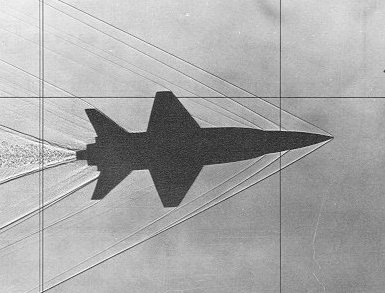
\includegraphics[width=\hsize]{../../skript/graphics/i-5-1.jpg}
\end{center}
\end{frame}

\begin{frame}
\frametitle{Mach-Kegel}
\begin{center}
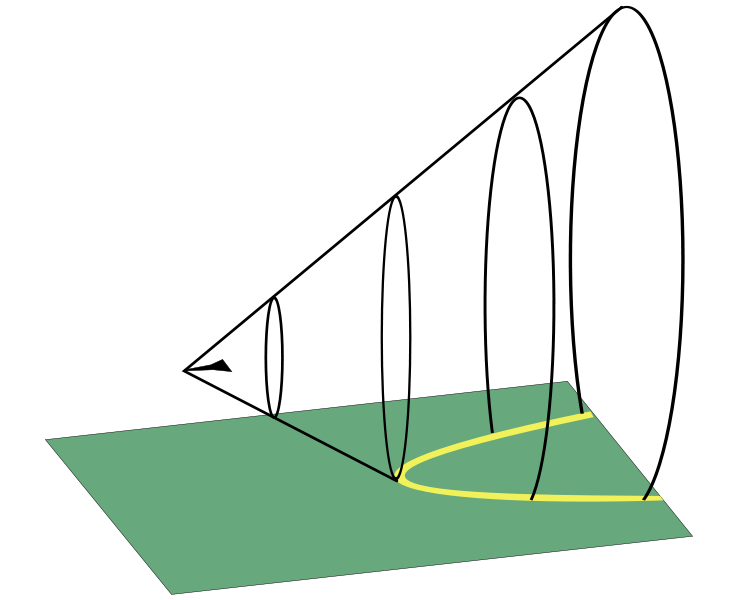
\includegraphics[width=0.8\hsize]{../../skript/graphics/shock.png}
\end{center}
\end{frame}

\begin{frame}
\frametitle{Mach-Kegel}
\begin{center}
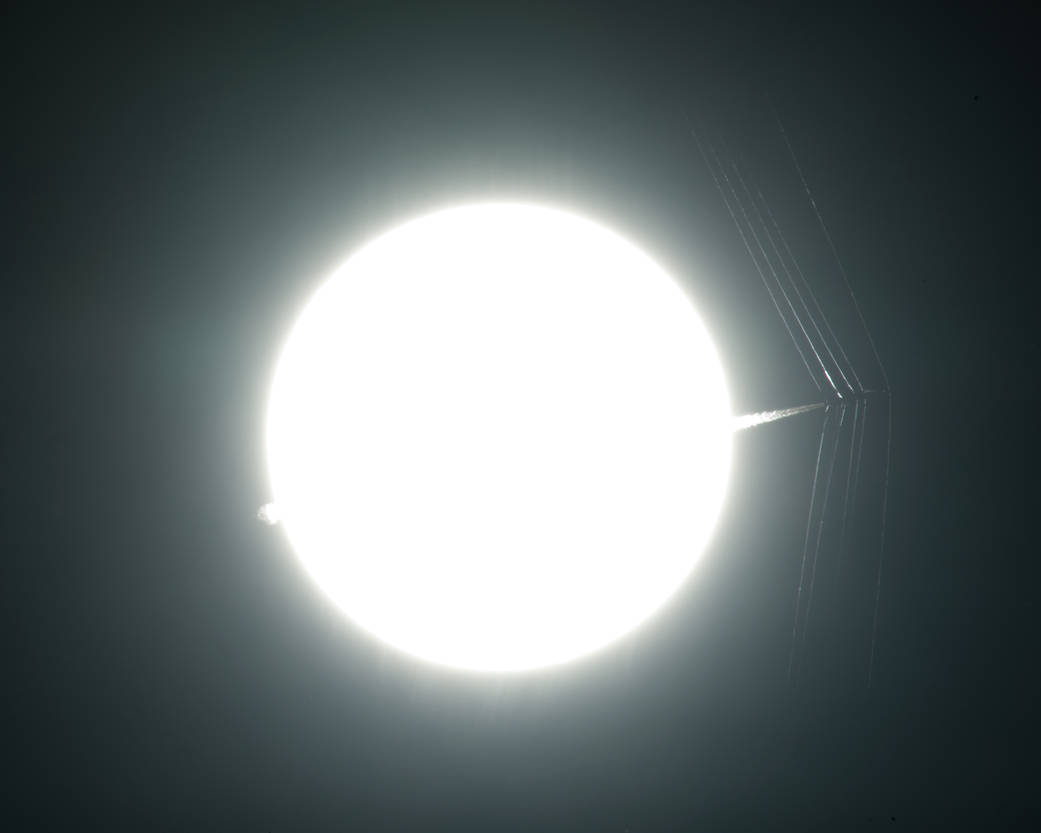
\includegraphics[width=\hsize]{afrc.jpg}
\end{center}
\end{frame}

\begin{frame}
\frametitle{Licht-Kegel}
\begin{center}
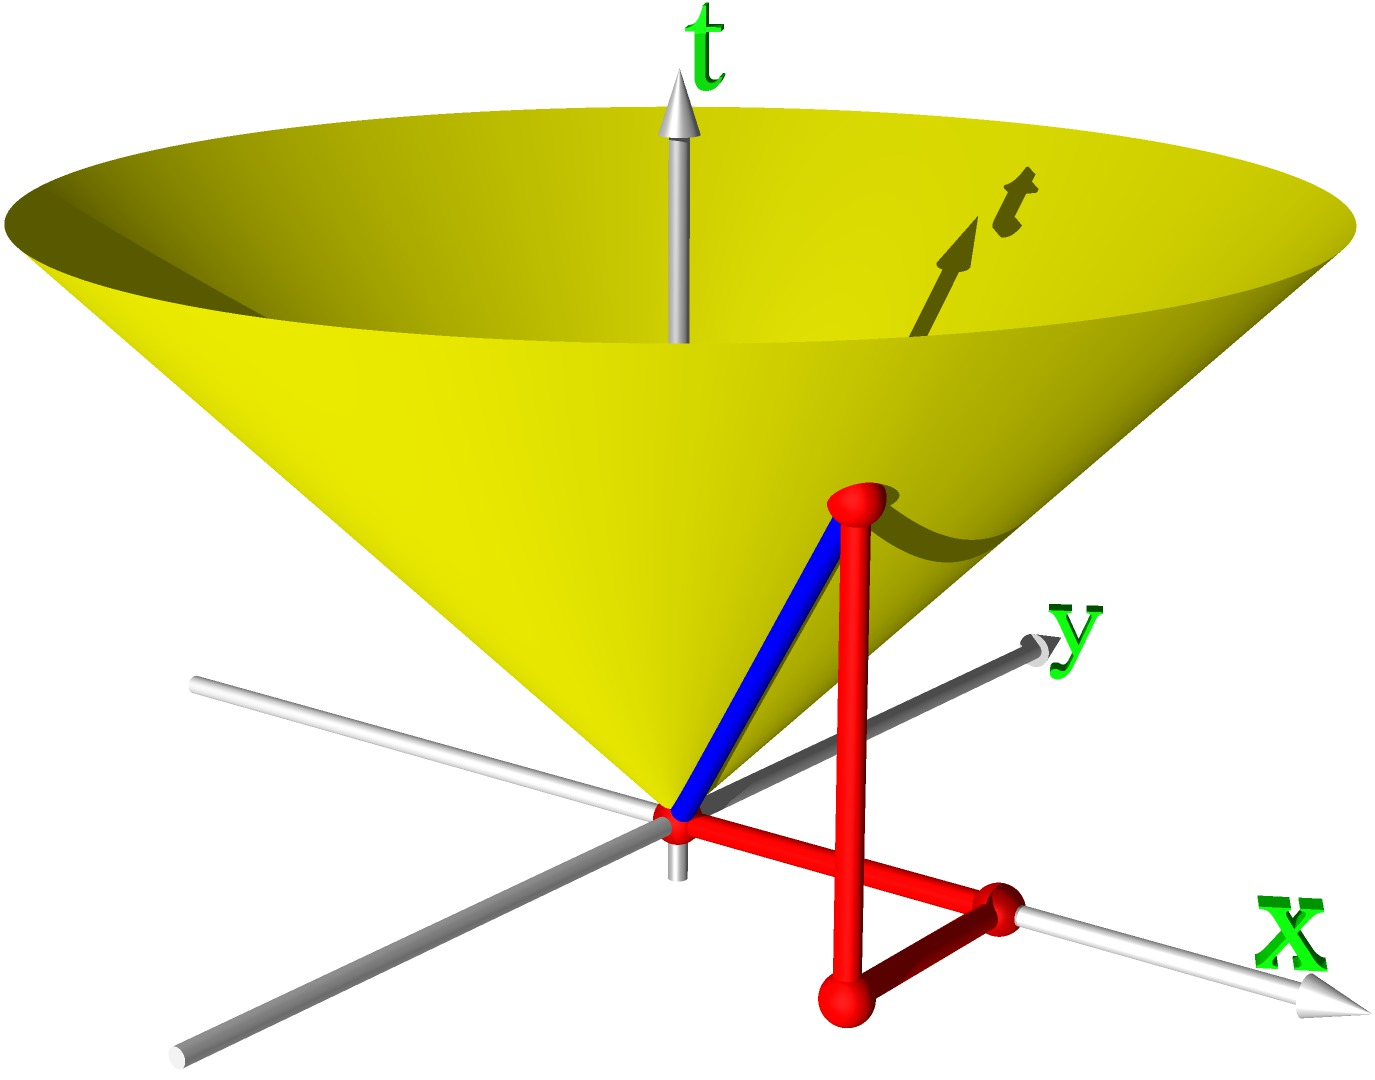
\includegraphics[width=\hsize]{lichtkegel.jpg}
\end{center}
\end{frame}

\begin{frame}
\frametitle{Parabolische PDGL}
\begin{center}
\includegraphics{../../skript/images/kausal-3.pdf}
\end{center}
\end{frame}

\begin{frame}
\begin{center}
\begin{tabular}{ccc}
\includegraphics[width=0.4\hsize]{../../skript/images/kausal-2.pdf}&&
\includegraphics[width=0.4\hsize]{../../skript/images/kausal-1.pdf}\\
\includegraphics[width=0.4\hsize]{../../skript/images/kausal-3.pdf}&&
\includegraphics[width=0.4\hsize]{../../skript/images/kausal-4.pdf}
\end{tabular}
\end{center}
\end{frame}
